%%%%%%%%%%%%%%%%%%%%%%%%%%%%%%%%%%%%%%%%%%%%%%
%                insertmeeting
% 1) Title (something creative & funny?)
% 2) Date (MM/DD/YYYY)
% 3) Location (ex. Hagerty High School)
% 4) People/Committees Present 
% 5) Picture 
% 6) Start Time & Stop Time (ex. 12:30AM to 4:30PM)
%%%%%%%%%%%%%%%%%%%%%%%%%%%%%%%%%%%%%%%%%%%%%%
\insertmeeting 
	{Meeting Example} 
	{11/18/21}
	{Hagerty High School}
	{Jensen}
	{Images/RobotPics/robot.jpg}
	{2:30 - 4:30}
	
\hhscommittee{General}
\noindent\hfil\rule{\textwidth}{.4pt}\hfil
\subsubsection*{Goals}
\begin{itemize}
    \item Watch kickoff
    \item Brainstorm   

\end{itemize} 

\noindent\hfil\rule{\textwidth}{.4pt}\hfil

\subsubsection*{Accomplishments}
Today, we watched the kickoff.
 

\begin{figure}[ht]
\centering
\begin{minipage}[b]{.48\textwidth}
  \centering
  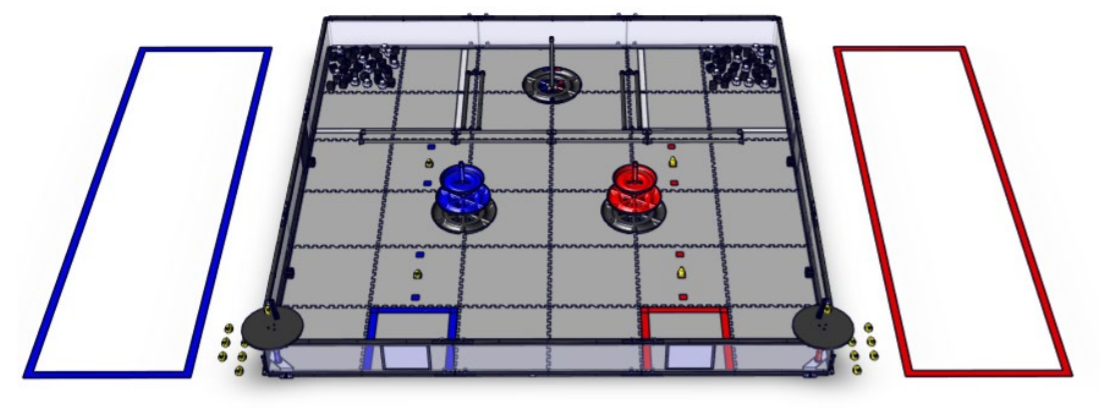
\includegraphics[width=0.95\textwidth]{Meetings/November/11-18-21/field.png}
  \caption{New Account in Github}
  \label{fig:pic1}
\end{minipage}%
\hfill%
\begin{minipage}[b]{.48\textwidth}
  \centering
  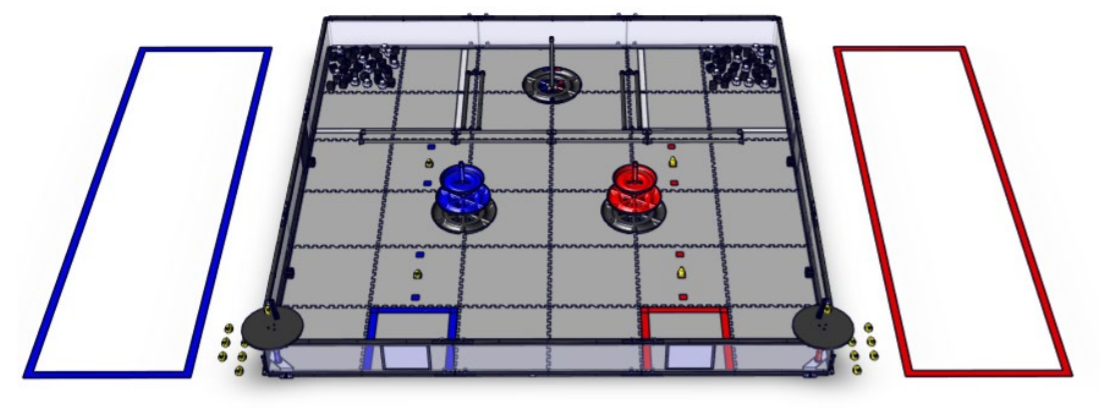
\includegraphics[width=0.95\textwidth]{Meetings/November/11-18-21/field.png}
  \caption{Screenshot of GitHub Repository}
  \label{fig:pic2}
\end{minipage}
\end{figure}

\begin{figure}[htp]
\centering
\includegraphics[width=0.95\textwidth, angle=0]{Meetings/November/11-01-21/defn_motor_plate.png}
\caption{Sketching the motor plate in the drive train skeleton}
\label{fig:pic3}
\end{figure}

Next, we needed a model of the Banebots gearbox in order to get the hole pattern. We made a motor assembly containing the gearbox, motor, and key as shown in Figure \ref{fig:banemod}. From there, we were able to create the motor plate part.

\begin{figure}[htp]
\centering
\includegraphics[width=0.95\textwidth, angle=0]{Meetings/November/11-01-21/bane_bot_motor.png}
\caption{Model of Banebots Planetary Gearbox and Motor}
\label{fig:banemod}
\end{figure}

In order to inherit the plate outline from the drive train skeleton, we performed the Copy Geometry operation, making the sketch and axises references embedded within the motor plate as shown in Figure \ref{fig:ext_mot}. From those references, we made an extrude for the plate, cutouts for the two motors to go into (Figure \ref{fig:motcutout}) and the slots for tensioning (Figure \ref{fig:slotten}). The two diagonal holes for the motor are larger than the other diagonal two because we wanted to be able to remove the motor from the plate without disassembling the gearbox form the motor (we are using the gearbox screws to mount the motor to the plate). As a result, two screws will already be tightened and their heads fit within the clearance holes and two screws will go through the motor plate and into the gearbox threads.

\whatsnext{
\begin{itemize}
    \item Laser cut intake parts
    \item 3d print intake parts
    \item Build intake
\end{itemize} 
}

